\documentclass{article}
\usepackage{graphicx}
\begin{document}
\hfill Alejandro Chavez

\hfill Lab 8 - Digital Logic

\hfill \today\\

\begin{center}\begin{large}Lab 8\end{large}\end{center}
\begin{itemize}
	\item
		1)\\
    Main:\\
    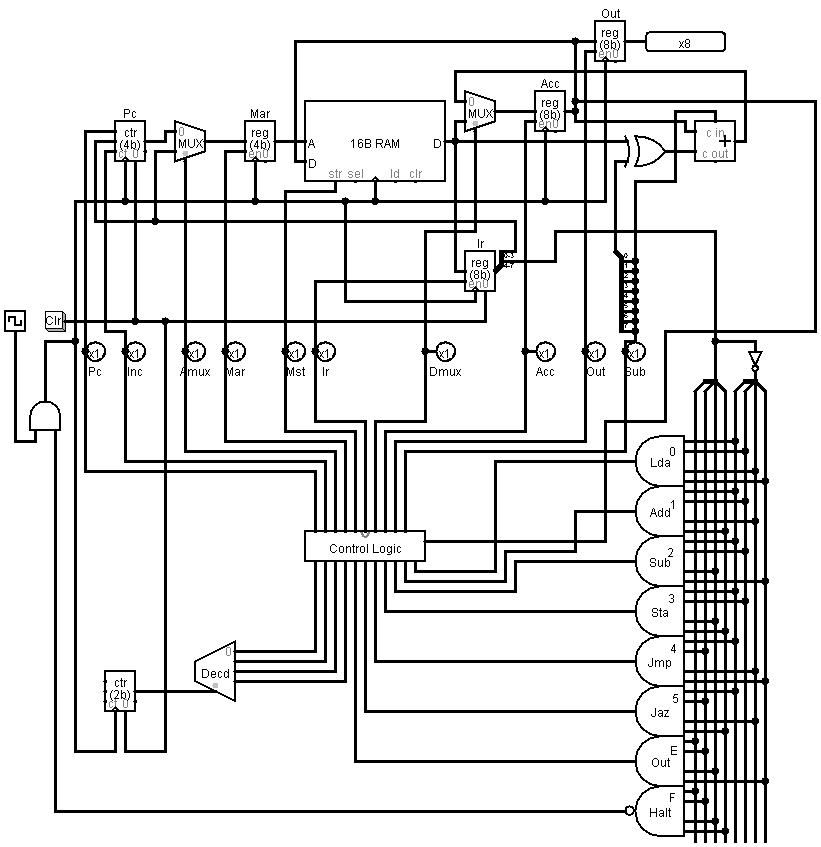
\includegraphics[scale=0.5]{lab8-main.png}\\
    Control Logic Component:\\
    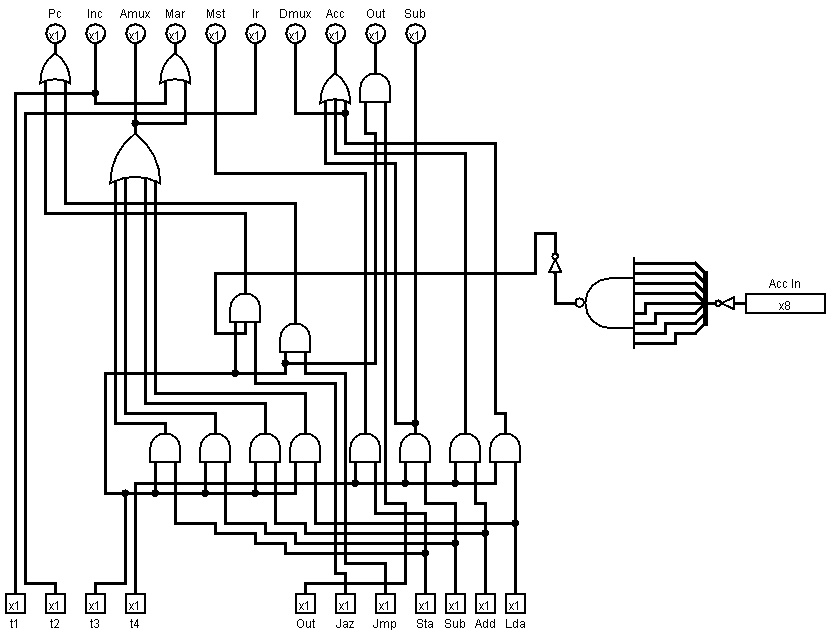
\includegraphics[scale=0.5]{lab8-clc.png}\\
    2)\\
    I loaded up the ram with the following instructions and data. As you can see it includes all of the available instructions.\\
    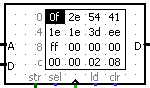
\includegraphics[scale=1]{snip1.PNG}\\
    After clocking it intil Halt, the result was this:\\
    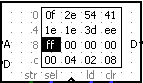
\includegraphics[scale=1]{snip2.PNG}\\
    And the output pin was four:\\
    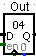
\includegraphics[scale=1]{snip3.PNG}\\
\end{itemize}
\end{document}
